\documentclass{article}
\usepackage[utf8]{inputenc}

% Page setup
\usepackage[a4paper,landscape,margin=2cm]{geometry}
\usepackage{amsmath}

% Typography
\usepackage[scaled]{helvet}
\let\familydefault\sfdefault

\usepackage[usenames,svgnames]{xcolor}
\usepackage{tikz,pgfplots}
\usetikzlibrary{positioning,arrows,intersections,calc}

\definecolor{coloractor}    {RGB}{199,212,104}
\definecolor{colormediator} {RGB}{ 79,142,209}
\definecolor{colorbus}      {RGB}{143,232,186}
\definecolor{colortext}     {RGB}{ 29, 29, 27}
\definecolor{coloraction}   {RGB}{129, 29, 27}
\definecolor{colortest}     {RGB}{ 69, 69,127}
\definecolor{colorrun}      {RGB}{127, 69, 69}

\begin{document}
\pagestyle{empty}
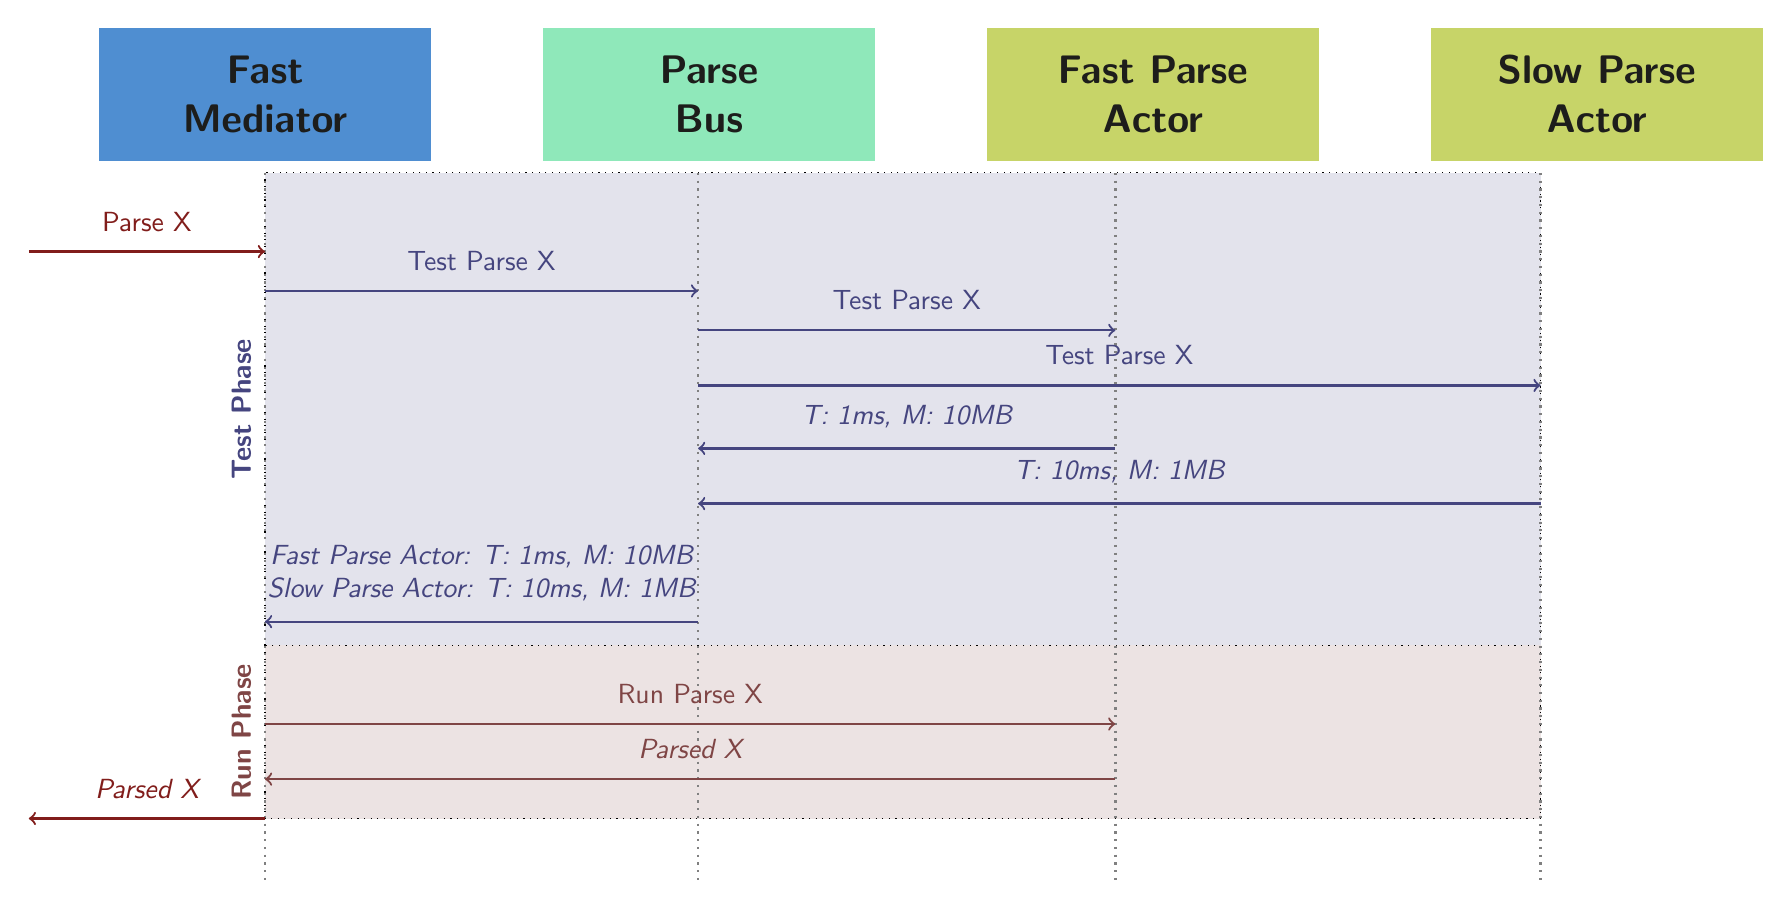
\begin{tikzpicture}[
    node distance = 4em, auto,
    font={\Large\itshape},
    base/.style={text=colortext,font={\Large\bfseries},inner sep=10pt,align=center,rectangle},
    txt/.style={text=colortext,font={},inner sep=7pt,align=center},
    action/.style={txt,color=coloraction},
    test/.style={txt,color=colortest},
    run/.style={txt,color=colorrun},
    treenode/.style={base,thick,draw=colortext,text width=2em},
    relation/.style={text width=13em},
    reply/.style={font={\itshape}},
]

    \node[base,fill=colormediator,text width=10em]                (mediator)  {Fast\\Mediator};
    \node[base,fill=colorbus,text width=10em,right=of mediator]   (bus)       {Parse\\Bus};
    \node[base,fill=coloractor,text width=10em,right=of bus]      (actor1)    {Fast Parse Actor};
    \node[base,fill=coloractor,text width=10em,right=of actor1]   (actor2)    {Slow Parse Actor};
    
    \draw[dotted,fill=colortest!15!white] (0,-1) rectangle (16.2,-7);
    \draw[dotted,fill=colorrun!15!white] (0,-7) rectangle (16.2,-9.2);
    
    \node[test,font={\bfseries},rotate=90] at (-0.3,-4) {Test Phase};
    \node[run,font={\bfseries},rotate=90] at (-0.3,-8.1) {Run Phase};
    
    \draw[thick,dotted,gray] (   0,-1) -- (   0,-10);
    \draw[thick,dotted,gray] ( 5.5,-1) -- ( 5.5,-10);
    \draw[thick,dotted,gray] (10.8,-1) -- (10.8,-10);
    \draw[thick,dotted,gray] (16.2,-1) -- (16.2,-10);
        

    \draw[action,->,thick] (-3,-2) -- (0,-2) node[midway,above] {Parse X};
    
    \draw[test,->,thick] (0,-2.5) -- (5.5,-2.5) node[midway,above] {Test Parse X};
    
    \draw[test,->,thick] (5.5,-3) -- (10.8,-3) node[midway,above] {Test Parse X};
    \draw[test,->,thick] (5.5,-3.7) -- (16.2,-3.7) node[midway,above] {Test Parse X};
    
    \draw[test,reply,<-,thick] (5.5,-4.5) -- (10.8,-4.5) node[midway,above] {T: 1ms, M: 10MB};
    \draw[test,reply,<-,thick] (5.5,-5.2) -- (16.2,-5.2) node[midway,above] {T: 10ms, M: 1MB};
    
    \draw[test,reply,<-,thick] (0,-6.7) -- (5.5,-6.7) node[midway,above] {Fast Parse Actor: T: 1ms, M: 10MB\\Slow Parse Actor: T: 10ms, M: 1MB};
    
    \draw[run,->,thick] (0,-8) -- (10.8,-8) node[midway,above] {Run Parse X};
    
    \draw[run,reply,<-,thick] (0,-8.7) -- (10.8,-8.7) node[midway,above] {Parsed X};
    
    \draw[action,reply,<-,thick] (-3,-9.2) -- (0,-9.2) node[midway,above] {Parsed X};

\end{tikzpicture}
\end{document}
